\documentclass[a4paper]{article}
\usepackage{praktikum}
\begin{document}
	
%%
%% Bitte das Deckblatt nicht verändern


\thispagestyle{empty}
\begin{center}

    {\large {\bf   BAI3-GKA WiSe2§ \\ Graphentheoretische Konzepte und Algorithmen \\[5mm]} }
    
{\huge Praktikumsaufgabe-Template  \\[5mm] Deckblatt}\\

\end{center}

				\begin{tabular}[t]{|r|l|}
				 \hline
%%%%				
%%%% Bitte  Ihren Namen und  Ihr Team und die Gruppe angeben
				GKA-Gruppe&                 \raisebox{-3mm}{\rule[8mm]{100mm}{0mm} }\\ \hline    
				Team &                                                        \\ \hline			
				& \textit{Iryna Trygub }               \\ \hline    
				& \textit{Ansgar Deuschel }               \\ \hline			
				& \textit{Kristoffer Schaaf }             \\ \hline  			
				\multicolumn{2}{c}{}\\  			
				\multicolumn{2}{l}{Bearbeitete Themen in Stichpunkten:}\\			
				\multicolumn{2}{c}{}\\  \hline
				Iryna Trygub &              \\ \hline    
				Ansgar Deuschel &                \\ \hline			
				Kristoffer Schaaf & Ops            \\ \hline 		
				\multicolumn{2}{c}{}\\  			
				\multicolumn{2}{l}{Geschätzte Arbeitszeiten in Stunden:}\\			
				\multicolumn{2}{c}{}\\  \hline
				Iryna Trygub &               \\ \hline    
				Ansgar Deuschel &                \\ \hline			
				Kristoffer Schaaf &               \\ \hline 			
				\end{tabular}
~\\[4mm]
		
		
\vfill


\newpage

\section{Einleitung}

\subsection{Dijkstra Algorithmus in Worten}

Wie genau funktioniert der Dijkstra Algorithmus und wo wird er angewendet?
Nehmen wir an Kreuzungen und Kreisverkehre seien Knoten und die Straßen, die diese verbinden die Kanten. Dann lässt sich bis auf Ausnahmen jedes Straßennetz durch einen Graphen darstellen. Um zu berechnen, wie Mensch am schnellsten von einem beliebigen Kreisverkehr zu einer beliebigen Kreuzung kommen kann, wird nun zum Beispiel der Dijkstra Algorithmus verwendet.

\begin{enumerate}
    \item Finden des Startknotens im Graphen.
    \item Dann die Distanz zu allen adjazenten Knoten berechnen und diese zusammen mit der Distanz zum Startknoten und den Knoten auf dem Weg dorthin in einer Open List speichern. 
    \item Den Ausgangsknoten auf eine Closed List verschieben, da alle inzidenten Kanten bearbeitet wurden.
    
    \item Nun den Knoten mit kürzester Distanz zum Startknoten in der Open List suchen und Schritt 2 von diesem Knoten aus wiederholen
    \begin{enumerate}
        \item Wenn ein Knoten, welcher bereits in der Open List gespeichert ist, erneut besucht wird, dann wird verglichen ob die neue Distanz kürzer ist. Wenn ja, wird der Knoten inklusive der Distanz zum Startknoten und den Knoten auf dem Weg dorthin aktualisiert. Wenn die Distanz länger ist, wird der Weg verworfen.
        \item Wenn alle inzidenten Kanten eines Knotens bearbeitet wurden, wird dieser Knoten in die Closed List verschoben.
    \end{enumerate}

    \item Der Algorithmus ist beendet, wenn entweder
    \begin{enumerate}
        \item alle Knoten des Graphen besucht wurden oder
        \item die Distanz vom Start- zum Zielknoten, die bisher kleinste gefundene Distanz ist.
    \end{enumerate}
\end{enumerate}

\subsection{Wählen des Grundansatzes}

Zur objektorientierten Abstrahierung eines Graphen gibt es zwei verschiedene Ansätze. Der erste Ansatz wäre, dass es einen Typ \textit{Kante} gibt, in welchem die vor- und nachfolgenden Knoten und die Länge der jeweiligen Kante gespeichert werden.\\
Diese Kanten würde dann den Graphen bilden und diesen in Form eines Sets darstellen:\\$Set <Kante> graph = new\ HashSet<>()$.\\
Problematisch wird es jetzt aber bereits zu Beginn des Dijkstra Algorithmus, wenn der Startknoten gefunden werden soll. Hat dieser immer den Grad 1, können wir über das Set \textit{graph} iterieren und stoppen, sobald der gesuchte Knoten in einer der Kanten enthalten ist. Ist der Grad des Startknoten aber größer 1, so muss über alle Kanten iteriert werden ob diese nicht mit dem Startknoten verbunden sind. Somit wäre schon der Start des Algorithmus ineffizient.

Der zweite Ansatz wäre die Kante als solches zu abstrahieren und nicht als eigenen Typen zu implementieren. Es gäbe dann nur den Typen Knoten, welcher alle benachbarten Knoten mit zugehöriger Distanz enthält.\\
Auch diese Knoten können nun in einem Set gespeichert werden:\\
$Set<Knoten> graph = new\ HashSet<>()$.\\
Bei der Suche nach dem Startknoten wird die Iteration gestoppt, sobald dieser gefunden wurde.
Somit ist der zweite Ansatz vorerst effizienter.

\subsection{Aufbau des Graphen}

Um den Dijkstra Algorithmus innerhalb eines Graphen anwenden zu können, muss zuerst ein Graph aufgebaut werden.
Wie im vorherigen Kapitel beschrieben, genügt es ein Set mit Knoten zu definieren.
Die Knoten des Graphen müssen folgende Informationen enthalten: Einen eindeutigen, im Graphen nur einmal vorkommenden Namen und die adjazenten Knoten.\\\\
Bedingungen, welche für den Graphen gelten:
\begin{itemize}
    \item Der Graph muss gewichtet sein und darf ausschließlich positive Kantengewichte haben.
    \item Der Graph kann unendlich viele Knoten besitzen.
    \item Allgemein kann Dijkstra auf einen gerichteten, ungerichteten oder gemischten Graphen angewendet werden. In dieser Implementierung wird aber ein ungerichteter Graph genutzt.
\end{itemize}

\subsection{Open und Closed List}

Knoten in der Closed List dienen der Kontrolle ob alle Kanten eines neu gefundenen Knoten bereits besucht wurden. Wird ein neuer Knoten gefunden, welcher noch nicht in der Open List enthalten ist, muss nun kontrolliert werden ob dieser bereits vollständig abgearbeitet ist, d.h. ob alle inzidenten Kanten bereits geprüft wurden.\\
Es reicht ein einfaches Set, welches die bereits besuchten Knoten enthält: $Set<Knoten>\ closedList$. Durch die Verwendung eines Sets wird außerdem das mehrfache Hinzufügen eines Knotens verhindert.\\\\
In der Open List wird der derzeitige Fortschritt festgehalten. Die verschiedenen Elemente können als Tabelleneintrag gespeichert werden. Eine Zeile dieser als Tabelle dargestellten Open List könnte folgendermaßen definiert werden:

\begin{table}[htbp]
    \centering
    \begin{tabular}{||l|l|l|l||}
    \hhline{|t:====:t|}
    \textbf{Beschreibung}   & Knoten  & Länge zum Startknoten & Knoten auf dem Weg    \\ \hhline{|----|}
    \textbf{Typ}            & Node    & Integer               & $List<Knoten>$        \\ \hhline{|----|}
    \textbf{Beispiel}       & ''D''   & 44                    & \{\{''A'', ... \},\{''C'', ... \}\}           \\ \hhline{|b:====:b|}
    \end{tabular}
    \caption{Open List}
\end{table}

\subsubsection{Open List als Set}

Auch wenn es dem Namen widerspricht, kann die Open List als Set implementiert werden. Wenn ein Knoten hinzugefügt wird, muss erst geschaut werden ob dieser schon vorhanden ist. Zum Vereinfachen dieser Suche wird eine Map genutzt: $Map<Knoten,\ Weg>\ openList$, wobei der Weg die Distanz zum Startknoten und die Knoten auf diesem Weg enthält. Wenn der Knoten nicht vorhanden ist, wird der Map ein neues Element hinzugefügt, welches als Key den neuen Knoten und als Value dessen Distanz zum Startknoten und den Knoten auf diesem Weg enthält.\\
Nach jeder Iteration muss der Knoten aus der Open List mit dem kürzestem Weg zum Startknoten bestimmt werden. Mit dieser Struktur ist dieser Prozess mit viel Rechenaufwand verbunden.

\subsubsection{Open List als Priority Queue} \label{priorityQueueSection}

Java bietet einen Typen Priority Queue an. Diesem kann eine Comparator übergeben werden, welcher die in der Queue enthaltenden Elemente nach bestimmten Attributen sortiert.\\
So können zum Beispiel verschiedene Listen mit Knoten beim Einfügen von Elementen direkt nach der in den Knoten enthaltenden Länge zum Startpunkt sortiert werden.\\
Ein großer Vorteil, den diese Implementierung mit sich bringt ist, dass durch die Funktion\\$PriorityQueue.peak()$ effizient der Knoten für die Wiederholung des Algorithmus bestimmt werden kann.\\
Der Typ Knoten muss des weiteren nur noch die adjazenten Knoten mit der Distanz enthalten.\\

\section{Dokumentation der Implementierung}

\subsection{Einführung neuer Typen}

Wie bereits in \ref{priorityQueueSection} beschrieben, ist die Implementierung der Open List als PriorityQueue am sinnvollsten.\\\\
Zur effizienteren Sortierung wird einer neuer Typ \textit{PriorityQueueItem} eingeführt. Zusätzlich wird der Typ \textit{Node} (auch Knoten) angepasst, wobei Teile eines bereits implementierten Nodes\footnote{\url{https://github.com/eugenp/tutorials/blob/master/algorithms-modules/algorithms-miscellaneous-2/src/main/java/com/baeldung/algorithms/ga/dijkstra/Node.java}} genutzt werden.\\

\begin{lstlisting}[language = java, frame = trBL]
@Data
@NoArgsContructor
public class PriorityQueueItem {

    /* Um das Item bei falscher Initialisierung nicht auf die
    erste Position in der PriorityQueue zu schieben, wird es mit einer
    maximalen Distanz initialisiert.*/
    private int distance = Integer.MAX_VALUE; 

    /*Die Reihenfolge dieser Knoten muss beibehalten werden,
    da ansonsten der kuerzeste Weg nachtraeglich nicht zurueckgegeben
    werden kann*/
    private List<Node> nodes = new LinkedList<>(); //Node -> Knoten
}

@Data
public class Node {
    
    private String name;
    
    Map<Node, Integer> adjacentNodes = new HashMap<>();

    public void addDestination(Node destination, int distance) {
        adjacentNodes.put(destination, distance);
    }
 
    public Node(String name) {
        this.name = name;
    }
}
\end{lstlisting}

\newpage
\subsection{Ablauf des Algorithmus mit einer Priority Queue}

\begin{enumerate}
    \item Ein leeres $Set<Node>\ closedList$ und eine leere $PriorityQueue<PriorityQueueItem> priorityQueue$ werden initialisiert.
    \item Für den Startknoten wird ein \textit{PriorityQueueItem} initialisiert und der \textit{priorityQueue} hinzugefügt. Dieses hat eine \textit{distance} von 0 und der \textit{nodes} Liste wird der Startknoten hinzugefügt.
    \item Jeder adjazente Knoten des Ausgangsknotens wird betrachtet:
    \begin{enumerate}
        \item Ist der Knoten bereits in der closedList: Knoten muss nicht weiter beachtet werden.
        \item Für jeden weiteren wird ein neues \textit{PriorityQueueItem} initialisiert. Die \textit{distance} ist die Distanz zwischen dem Ausgangsknoten und dessen adjazentem Knoten. Die \textit{nodes} Liste enthält den neuen Knoten.\\Diese neuen \textit{PriorityQueueItems} werden nun jeweils mit dem bereits bestehendem \textit{PriorityQueueItem} des Ausgangsknotens ergänzt. Hierbei werden die Distanzen aufsummiert und die Listen konkateniert (Reihenfolge beachten).
    \end{enumerate}
    \item Die neu entstandenen \textit{PriorityQueueItems} ersetzen nun das \textit{PriorityQueueItem} des Ausgangsknotens in der \textit{PriorityQueue} unter folgender Bedingung:
    \begin{enumerate}
         \item Ist der letzte Knoten aus der \textit{nodes} Liste einer dieser \textit{PriorityQueueItems} bereits das letzte Element einer \textit{nodes} Liste eines \textit{PriorityQueueItems} in der \textit{PriorityQueue} muss verglichen werden, welche \textit{distance} der \textit{PriorityQueueItems} kleiner ist und nur dieses \textit{PriorityQueueItem} wird behalten.
    \end{enumerate}
    \item Da alle Kanten des Ausgangsknotens jetzt untersucht wurden, wird dieser der \textit{closedList} hinzugefügt.
    \item Das oberste Element der \textit{PriorityQueue} wird bestimmt. Das letzte Element aus dessen \textit{nodes} Liste wird zum neuen Ausgangsknoten und Schritt 3 wird wiederholt.
    \item Der Algorithmus ist beendet, wenn entweder
    \begin{enumerate}
        \item alle Knoten des Graphen besucht wurden oder
        \item der Zielknoten das letzte Element der \textit{nodes} Liste eines bereits in der \textit{PriorityQueue} enthaltendem \textit{PriorityQueueItem} und die \textit{distance} die bisher kleinste gefundene Distanz ist.
    \end{enumerate}
\end{enumerate}

\begin{figure}[htbp]
	\centering
		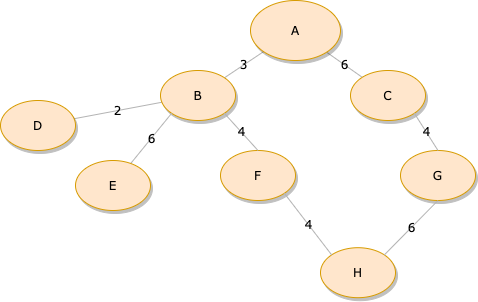
\includegraphics[width=0.60\textwidth]{Latex/Figs/Beispielgraph_2.png}		
	\caption{Gewichteter, ungerichteter Graph}
	\label{fig:beispielgraph_2}
\end{figure}

\subsubsection{Beispiel}

Sei der Knoten ''A'' auf folgendem Graphen~\ref{fig:beispielgraph_2} ein Startknoten.
Nach zwei Iterationen sieht der Inhalt der PriorityQueue wie folgt aus:\\

\begin{lstlisting}[language = java, frame = trBL]
priorityQueue = {
    {5, {A, B, D}},
    {6, {A, C}},
    {7, {A, B, F}},
    {9, {A, B, E}}
};

closedList = { };
\end{lstlisting}



\newpage

\section{Nachwort}

\subsection{Dijkstra als Baum}

Eine weitere Möglichkeit den Algorithmus zu implementieren wäre es die besuchten Knoten als Baum nachzubauen, während der originale Graph bearbeitet wird. Der Startknoten ist nun der Elternknoten, während nach der ersten Iteration alle adjazenten Knoten die Kinderknoten sind. 

\cite{KN2012} 
und Ihre Abbildungen nicht, z.B. Abb.~\ref{fig:bild}.
  

\section{Beantwortung der  Fragen}
\begin{enumerate}
						\item Antwort auf die erste Frage
						\item 
					\end{enumerate}


\bibliographystyle{alpha}
\bibliography{mybib}
%%%%GKA_PR_template.tex

\documentclass[a4paper]{article}
\usepackage{praktikum}
\begin{document}
	
%%
%% Bitte das Deckblatt nicht verändern


\thispagestyle{empty}
\begin{center}

    {\large {\bf   BAI3-GKA WiSe2§ \\ Graphentheoretische Konzepte und Algorithmen \\[5mm]} }
    
{\huge Praktikumsaufgabe-Template  \\[5mm] Deckblatt}\\

\end{center}

				\begin{tabular}[t]{|r|l|}
				 \hline
%%%%				
%%%% Bitte  Ihren Namen und  Ihr Team und die Gruppe angeben
				GKA-Gruppe&                 \raisebox{-3mm}{\rule[8mm]{100mm}{0mm} }\\ \hline    
				Team &                                                        \\ \hline			
				& \textit{Iryna Trygub }               \\ \hline    
				& \textit{Ansgar Deuschel }               \\ \hline			
				& \textit{Kristoffer Schaaf }             \\ \hline  			
				\multicolumn{2}{c}{}\\  			
				\multicolumn{2}{l}{Bearbeitete Themen in Stichpunkten:}\\			
				\multicolumn{2}{c}{}\\  \hline
				Iryna Trygub &              \\ \hline    
				Ansgar Deuschel &                \\ \hline			
				Kristoffer Schaaf & Ops            \\ \hline 		
				\multicolumn{2}{c}{}\\  			
				\multicolumn{2}{l}{Geschätzte Arbeitszeiten in Stunden:}\\			
				\multicolumn{2}{c}{}\\  \hline
				Iryna Trygub &               \\ \hline    
				Ansgar Deuschel &                \\ \hline			
				Kristoffer Schaaf &               \\ \hline 			
				\end{tabular}
~\\[4mm]
		
		
\vfill


\newpage

\section{Einleitung}

\subsection{Vorab}

Angenommen, der Dijkstra Algorithmus wäre in zwei Ansätzen zu lösen. Dann wären der erste Ansatz, dass es einen Typ Kante gibt, in welchem die Vor- und Nachfolgenden Knoten und die Länge der jeweiligen Kante gespeichert werden.\\
Diese Kanten würde dann den Graphen bilden und diesen in Form eines Sets darstellen:\\$Set <Kante> graph = new\ HashSet<>()$.\\
Problematisch wird es jetzt allerdings schon, wenn der Startknoten gefunden werden soll. Hat dieser immer den Grad 1, können wir über das Set graph iterieren und stoppen, sobald der gesuchte Knoten in einer der Kanten enthalten ist. Ist der Grad des Startknoten allerdings größer 1, so muss über alle Kanten iteriert werden ob diese nicht mit dem Startknoten verbunden sind. Somit wäre schon der Start des Algorithmus ineffizient.

Der zweite Ansatz auf welchem auch folgende Implementierung\footnote{\url{https://github.com/eugenp/tutorials/blob/master/algorithms-modules/algorithms-miscellaneous-2/src/main/java/com/baeldung/algorithms/ga/dijkstra/Node.java}} basiert wäre, die Kante als solches zu abstrahieren und nicht als eigenen Typen zu implementieren. Es gäbe dann nur den Typen Knoten, welcher alle benachbarten Knoten mit zugehöriger Distanz enthält.\\
Auch diese Knoten können nun in einem Set gespeichert werden:\\
$Set<Knoten> graph = new\ HashSet<>()$.\\
Allerdings wird bei der Suche nach dem Startknoten die Iteration gestoppt, sobald dieser gefunden wurde.
Somit ist der zweite Ansatz vorerst effizienter.

\subsection{Aufbau des Graphen}

Um den Dijkstra Algorithmus innerhalb eines Graphen anwenden zu können, muss zuerst ein Graph aufgebaut werden.
Wie im vorherigen Kapitel beschrieben, genügt es ein Set mit Knoten zu definieren.
Die Knoten des Graphen müssen folgende Informationen enthalten: Einen eindeutigen, im Graphen nur einmal vorkommenden, Namen und die adjazenten Knoten. Letztere werden in Form einer Map definiert, da so der Knoten mit inzidenter Kante und dessen Länge sinnvoll zusammen gespeichert wird.

Bedingungen, welche für den Graphen gelten:
- Der Graph muss gewichtet sein und darf ausschließlich positive Kantengewichte haben
- Der Graph kann unendlich viele Knoten besitzen
- Allgemein kann Dijkstra auf einen gerichteten, ungerichteten oder gemischten Graphen angewendet werden. In dieser Implementierung wird aber ein ungerichteter Graph genutzt.

\subsection{Dijkstra Algorithmus in Worten}

Wie genau funktioniert der Dijkstra Algorithmus aber eigentlich und wo wird er angewendet?
Nehmen wir an Kreuzungen und Kreisverkehre seien Knoten und die Straßen, die diese verbinden die Kanten. Dann lässt sich bis auf Ausnahmen jedes Straßennetz durch einen Graphen darstellen. Um zu berechnen, wie Mensch am schnellsten von einem beliebigen Kreisverkehr zu einer beliebigen Kreuzung kommen kann, wird nur zum Beispiel der Dijkstra Algorithmus verwendet.

\begin{enumerate}
    \item Finden des Startknotens im Graphen.
    \item Dann die Distanz zu allen benachbarten Knoten berechnen und diese zusammen mit der Distanz zum Startknoten und den Knoten auf dem Weg dorthin in einer Open List speichern
    
    \item Nun den Knoten mit kürzester Distanz zum Startknoten in Open List suchen und Schritt 2 von diesem Knoten aus wiederholen
    \begin{enumerate}
        \item Wenn ein Knoten, welcher bereits in der Open List gespeichert ist, erneut besucht wird, wird verglichen ob die neue Distanz kürzer ist. Wenn ja, wird der Knoten inklusive der Distanz zum Startknoten und den Knoten auf dem Weg dorthin aktualisiert. Wenn die Distanz länger ist, wird der Weg verworfen.
        \item Wenn alle inzidenten Kanten eines Knotens bearbeitet wurden, wird dieser Knoten in die Closed List verschoben.
    \end{enumerate}

    \item Der Algorithmus ist beendet, wenn entweder
    \begin{enumerate}
        \item alle Knoten des Graphen besucht wurden oder
        \item die Distanz vom Start- zum Zielknoten, die bisher kleinste gefundene Distanz ist.
    \end{enumerate}
    
\end{enumerate}

\subsection{Elemente}

Die benötigten Elemente, bzw. Typen sind 

\section{Dokumentation Ihrer Implementierung}

\newpage

\cite{KN2012} 
und Ihre Abbildungen nicht, z.B. Abb.~\ref{fig:bild}.
  

\section{Beantwortung der  Fragen}
\begin{enumerate}
						\item Antwort auf die erste Frage
						\item 
					\end{enumerate}


\section*{Abbildungen}


\begin{figure}[h]
	\centering
		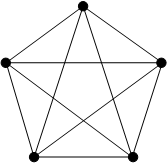
\includegraphics[width=0.50\textwidth]{Figs/Bild.png}		
	\caption{Beispiel für eine Abbildung}
	\label{fig:bild}
\end{figure}



\bibliographystyle{alpha}
\bibliography{mybib}
%%%%GKA_PR_template.tex

\documentclass[a4paper]{article}
\usepackage{praktikum}
\begin{document}
	
%%
%% Bitte das Deckblatt nicht verändern


\thispagestyle{empty}
\begin{center}

    {\large {\bf   BAI3-GKA WiSe2§ \\ Graphentheoretische Konzepte und Algorithmen \\[5mm]} }
    
{\huge Praktikumsaufgabe-Template  \\[5mm] Deckblatt}\\

\end{center}

				\begin{tabular}[t]{|r|l|}
				 \hline
%%%%				
%%%% Bitte  Ihren Namen und  Ihr Team und die Gruppe angeben
				GKA-Gruppe&                 \raisebox{-3mm}{\rule[8mm]{100mm}{0mm} }\\ \hline    
				Team &                                                        \\ \hline			
				& \textit{Iryna Trygub }               \\ \hline    
				& \textit{Ansgar Deuschel }               \\ \hline			
				& \textit{Kristoffer Schaaf }             \\ \hline  			
				\multicolumn{2}{c}{}\\  			
				\multicolumn{2}{l}{Bearbeitete Themen in Stichpunkten:}\\			
				\multicolumn{2}{c}{}\\  \hline
				Iryna Trygub &              \\ \hline    
				Ansgar Deuschel &                \\ \hline			
				Kristoffer Schaaf & Ops            \\ \hline 		
				\multicolumn{2}{c}{}\\  			
				\multicolumn{2}{l}{Geschätzte Arbeitszeiten in Stunden:}\\			
				\multicolumn{2}{c}{}\\  \hline
				Iryna Trygub &               \\ \hline    
				Ansgar Deuschel &                \\ \hline			
				Kristoffer Schaaf &               \\ \hline 			
				\end{tabular}
~\\[4mm]
		
		
\vfill


\newpage

\section{Einleitung}

\subsection{Vorab}

Angenommen, der Dijkstra Algorithmus wäre in zwei Ansätzen zu lösen. Dann wären der erste Ansatz, dass es einen Typ Kante gibt, in welchem die Vor- und Nachfolgenden Knoten und die Länge der jeweiligen Kante gespeichert werden.\\
Diese Kanten würde dann den Graphen bilden und diesen in Form eines Sets darstellen:\\$Set <Kante> graph = new\ HashSet<>()$.\\
Problematisch wird es jetzt allerdings schon, wenn der Startknoten gefunden werden soll. Hat dieser immer den Grad 1, können wir über das Set graph iterieren und stoppen, sobald der gesuchte Knoten in einer der Kanten enthalten ist. Ist der Grad des Startknoten allerdings größer 1, so muss über alle Kanten iteriert werden ob diese nicht mit dem Startknoten verbunden sind. Somit wäre schon der Start des Algorithmus ineffizient.

Der zweite Ansatz auf welchem auch folgende Implementierung\footnote{\url{https://github.com/eugenp/tutorials/blob/master/algorithms-modules/algorithms-miscellaneous-2/src/main/java/com/baeldung/algorithms/ga/dijkstra/Node.java}} basiert wäre, die Kante als solches zu abstrahieren und nicht als eigenen Typen zu implementieren. Es gäbe dann nur den Typen Knoten, welcher alle benachbarten Knoten mit zugehöriger Distanz enthält.\\
Auch diese Knoten können nun in einem Set gespeichert werden:\\
$Set<Knoten> graph = new\ HashSet<>()$.\\
Allerdings wird bei der Suche nach dem Startknoten die Iteration gestoppt, sobald dieser gefunden wurde.
Somit ist der zweite Ansatz vorerst effizienter.

\subsection{Aufbau des Graphen}

Um den Dijkstra Algorithmus innerhalb eines Graphen anwenden zu können, muss zuerst ein Graph aufgebaut werden.
Wie im vorherigen Kapitel beschrieben, genügt es ein Set mit Knoten zu definieren.
Die Knoten des Graphen müssen folgende Informationen enthalten: Einen eindeutigen, im Graphen nur einmal vorkommenden, Namen und die adjazenten Knoten. Letztere werden in Form einer Map definiert, da so der Knoten mit inzidenter Kante und dessen Länge sinnvoll zusammen gespeichert wird.

Bedingungen, welche für den Graphen gelten:
- Der Graph muss gewichtet sein und darf ausschließlich positive Kantengewichte haben
- Der Graph kann unendlich viele Knoten besitzen
- Allgemein kann Dijkstra auf einen gerichteten, ungerichteten oder gemischten Graphen angewendet werden. In dieser Implementierung wird aber ein ungerichteter Graph genutzt.

\subsection{Dijkstra Algorithmus in Worten}

Wie genau funktioniert der Dijkstra Algorithmus aber eigentlich und wo wird er angewendet?
Nehmen wir an Kreuzungen und Kreisverkehre seien Knoten und die Straßen, die diese verbinden die Kanten. Dann lässt sich bis auf Ausnahmen jedes Straßennetz durch einen Graphen darstellen. Um zu berechnen, wie Mensch am schnellsten von einem beliebigen Kreisverkehr zu einer beliebigen Kreuzung kommen kann, wird nur zum Beispiel der Dijkstra Algorithmus verwendet.

\begin{enumerate}
    \item Finden des Startknotens im Graphen.
    \item Dann die Distanz zu allen benachbarten Knoten berechnen und diese zusammen mit der Distanz zum Startknoten und den Knoten auf dem Weg dorthin in einer Open List speichern
    
    \item Nun den Knoten mit kürzester Distanz zum Startknoten in Open List suchen und Schritt 2 von diesem Knoten aus wiederholen
    \begin{enumerate}
        \item Wenn ein Knoten, welcher bereits in der Open List gespeichert ist, erneut besucht wird, wird verglichen ob die neue Distanz kürzer ist. Wenn ja, wird der Knoten inklusive der Distanz zum Startknoten und den Knoten auf dem Weg dorthin aktualisiert. Wenn die Distanz länger ist, wird der Weg verworfen.
        \item Wenn alle inzidenten Kanten eines Knotens bearbeitet wurden, wird dieser Knoten in die Closed List verschoben.
    \end{enumerate}

    \item Der Algorithmus ist beendet, wenn entweder
    \begin{enumerate}
        \item alle Knoten des Graphen besucht wurden oder
        \item die Distanz vom Start- zum Zielknoten, die bisher kleinste gefundene Distanz ist.
    \end{enumerate}
    
\end{enumerate}

\subsection{Elemente}

Die benötigten Elemente, bzw. Typen sind 

\section{Dokumentation Ihrer Implementierung}

\newpage

\cite{KN2012} 
und Ihre Abbildungen nicht, z.B. Abb.~\ref{fig:bild}.
  

\section{Beantwortung der  Fragen}
\begin{enumerate}
						\item Antwort auf die erste Frage
						\item 
					\end{enumerate}


\section*{Abbildungen}


\begin{figure}[h]
	\centering
		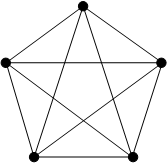
\includegraphics[width=0.50\textwidth]{Figs/Bild.png}		
	\caption{Beispiel für eine Abbildung}
	\label{fig:bild}
\end{figure}



\bibliographystyle{alpha}
\bibliography{mybib}
%%%%GKA_PR_template.tex

\documentclass[a4paper]{article}
\usepackage{praktikum}
\begin{document}
	
\input{deckblatt}
\newpage

\section{Einleitung}

\subsection{Vorab}

Angenommen, der Dijkstra Algorithmus wäre in zwei Ansätzen zu lösen. Dann wären der erste Ansatz, dass es einen Typ Kante gibt, in welchem die Vor- und Nachfolgenden Knoten und die Länge der jeweiligen Kante gespeichert werden.\\
Diese Kanten würde dann den Graphen bilden und diesen in Form eines Sets darstellen:\\$Set <Kante> graph = new\ HashSet<>()$.\\
Problematisch wird es jetzt allerdings schon, wenn der Startknoten gefunden werden soll. Hat dieser immer den Grad 1, können wir über das Set graph iterieren und stoppen, sobald der gesuchte Knoten in einer der Kanten enthalten ist. Ist der Grad des Startknoten allerdings größer 1, so muss über alle Kanten iteriert werden ob diese nicht mit dem Startknoten verbunden sind. Somit wäre schon der Start des Algorithmus ineffizient.

Der zweite Ansatz auf welchem auch folgende Implementierung\footnote{\url{https://github.com/eugenp/tutorials/blob/master/algorithms-modules/algorithms-miscellaneous-2/src/main/java/com/baeldung/algorithms/ga/dijkstra/Node.java}} basiert wäre, die Kante als solches zu abstrahieren und nicht als eigenen Typen zu implementieren. Es gäbe dann nur den Typen Knoten, welcher alle benachbarten Knoten mit zugehöriger Distanz enthält.\\
Auch diese Knoten können nun in einem Set gespeichert werden:\\
$Set<Knoten> graph = new\ HashSet<>()$.\\
Allerdings wird bei der Suche nach dem Startknoten die Iteration gestoppt, sobald dieser gefunden wurde.
Somit ist der zweite Ansatz vorerst effizienter.

\subsection{Aufbau des Graphen}

Um den Dijkstra Algorithmus innerhalb eines Graphen anwenden zu können, muss zuerst ein Graph aufgebaut werden.
Wie im vorherigen Kapitel beschrieben, genügt es ein Set mit Knoten zu definieren.
Die Knoten des Graphen müssen folgende Informationen enthalten: Einen eindeutigen, im Graphen nur einmal vorkommenden, Namen und die adjazenten Knoten. Letztere werden in Form einer Map definiert, da so der Knoten mit inzidenter Kante und dessen Länge sinnvoll zusammen gespeichert wird.

Bedingungen, welche für den Graphen gelten:
- Der Graph muss gewichtet sein und darf ausschließlich positive Kantengewichte haben
- Der Graph kann unendlich viele Knoten besitzen
- Allgemein kann Dijkstra auf einen gerichteten, ungerichteten oder gemischten Graphen angewendet werden. In dieser Implementierung wird aber ein ungerichteter Graph genutzt.

\subsection{Dijkstra Algorithmus in Worten}

Wie genau funktioniert der Dijkstra Algorithmus aber eigentlich und wo wird er angewendet?
Nehmen wir an Kreuzungen und Kreisverkehre seien Knoten und die Straßen, die diese verbinden die Kanten. Dann lässt sich bis auf Ausnahmen jedes Straßennetz durch einen Graphen darstellen. Um zu berechnen, wie Mensch am schnellsten von einem beliebigen Kreisverkehr zu einer beliebigen Kreuzung kommen kann, wird nur zum Beispiel der Dijkstra Algorithmus verwendet.

\begin{enumerate}
    \item Finden des Startknotens im Graphen.
    \item Dann die Distanz zu allen benachbarten Knoten berechnen und diese zusammen mit der Distanz zum Startknoten und den Knoten auf dem Weg dorthin in einer Open List speichern
    
    \item Nun den Knoten mit kürzester Distanz zum Startknoten in Open List suchen und Schritt 2 von diesem Knoten aus wiederholen
    \begin{enumerate}
        \item Wenn ein Knoten, welcher bereits in der Open List gespeichert ist, erneut besucht wird, wird verglichen ob die neue Distanz kürzer ist. Wenn ja, wird der Knoten inklusive der Distanz zum Startknoten und den Knoten auf dem Weg dorthin aktualisiert. Wenn die Distanz länger ist, wird der Weg verworfen.
        \item Wenn alle inzidenten Kanten eines Knotens bearbeitet wurden, wird dieser Knoten in die Closed List verschoben.
    \end{enumerate}

    \item Der Algorithmus ist beendet, wenn entweder
    \begin{enumerate}
        \item alle Knoten des Graphen besucht wurden oder
        \item die Distanz vom Start- zum Zielknoten, die bisher kleinste gefundene Distanz ist.
    \end{enumerate}
    
\end{enumerate}

\subsection{Elemente}

Die benötigten Elemente, bzw. Typen sind 

\section{Dokumentation Ihrer Implementierung}

\newpage

\cite{KN2012} 
und Ihre Abbildungen nicht, z.B. Abb.~\ref{fig:bild}.
  

\section{Beantwortung der  Fragen}
\begin{enumerate}
						\item Antwort auf die erste Frage
						\item 
					\end{enumerate}


\section*{Abbildungen}


\begin{figure}[h]
	\centering
		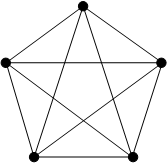
\includegraphics[width=0.50\textwidth]{Figs/Bild.png}		
	\caption{Beispiel für eine Abbildung}
	\label{fig:bild}
\end{figure}



\bibliographystyle{alpha}
\bibliography{mybib}
%\include{GKA_PR_template.bbl}

\end{document}

\end{document}

\end{document}

\end{document}